\section{並列計算とは}

\begin{frame}[t,fragile]{Richardson's Forecast Factory (1922)}
  \resizebox{.8\textwidth}{!}{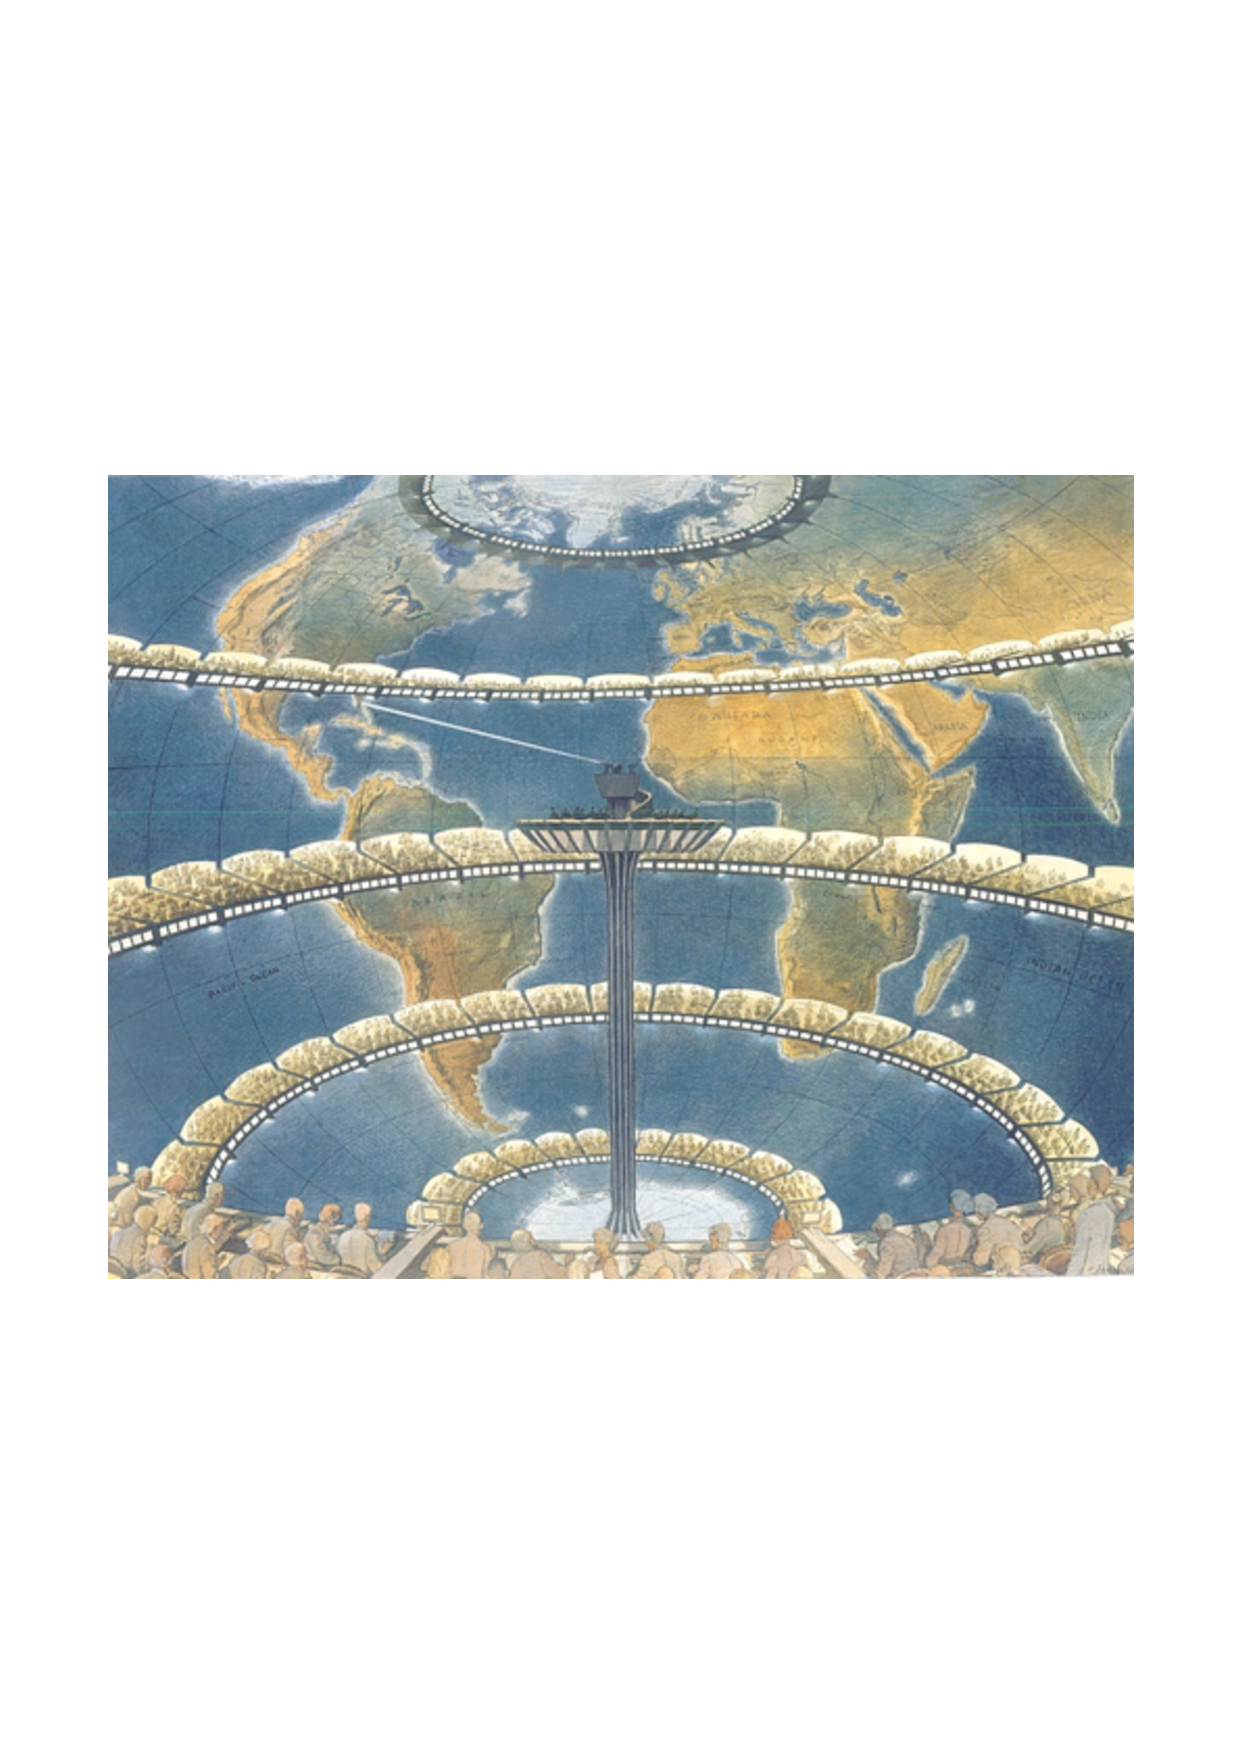
\includegraphics{image/SchuitenHD3.pdf}}
\end{frame}

\begin{frame}[t,fragile]{並列化とは何か}
  \begin{itemize}
    \setlength{\itemsep}{1em}
  \item 目的: シミュレーションをできる限り「短時間」で終了させる
    \begin{itemize}
      \item たとえ総CPU時間が伸びても「ターンアラウンド時間」を短かくしたい
      \item 一台のパソコンでは100年かかる計算を学位論文に間に合わせたい
      \item 今の100倍の精度の計算を同じ「実時間」で実行したい
    \end{itemize}
  \item 並列化とは
    \begin{enumerate}
    \item CPUの行なうべき仕事を複数の小さな仕事に分割
    \item それらを複数のCPUで同時実行
    \end{enumerate}
  \item うまく並列化を行なうために必要なこと
    \begin{enumerate}
    \item プログラムのどの部分をどのように並列化すればより効果的かを理解する
    \item 並列化を実装するにはどのようにプログラムを書けば良いかを理解する
    \end{enumerate}
  \end{itemize}
\end{frame}

\begin{frame}[t,fragile]{並列計算の原理}
  \begin{itemize}
    %\setlength{\itemsep}{1em}
  \item ノードは、互いに必要な情報を交換しながら、それぞれ異なる処理をしなければならない
  \item ノード毎に異なる指示(= プログラム)を与えるのは大変 (特にノード数が何万もの場合)
  \item 一つのプログラムでノード(ランクとも呼ばれる)毎に異なる指示を与えたい

    ⇒ SPMD (Single Program, Multiple Data streams)

    \resizebox{.9\textwidth}{!}{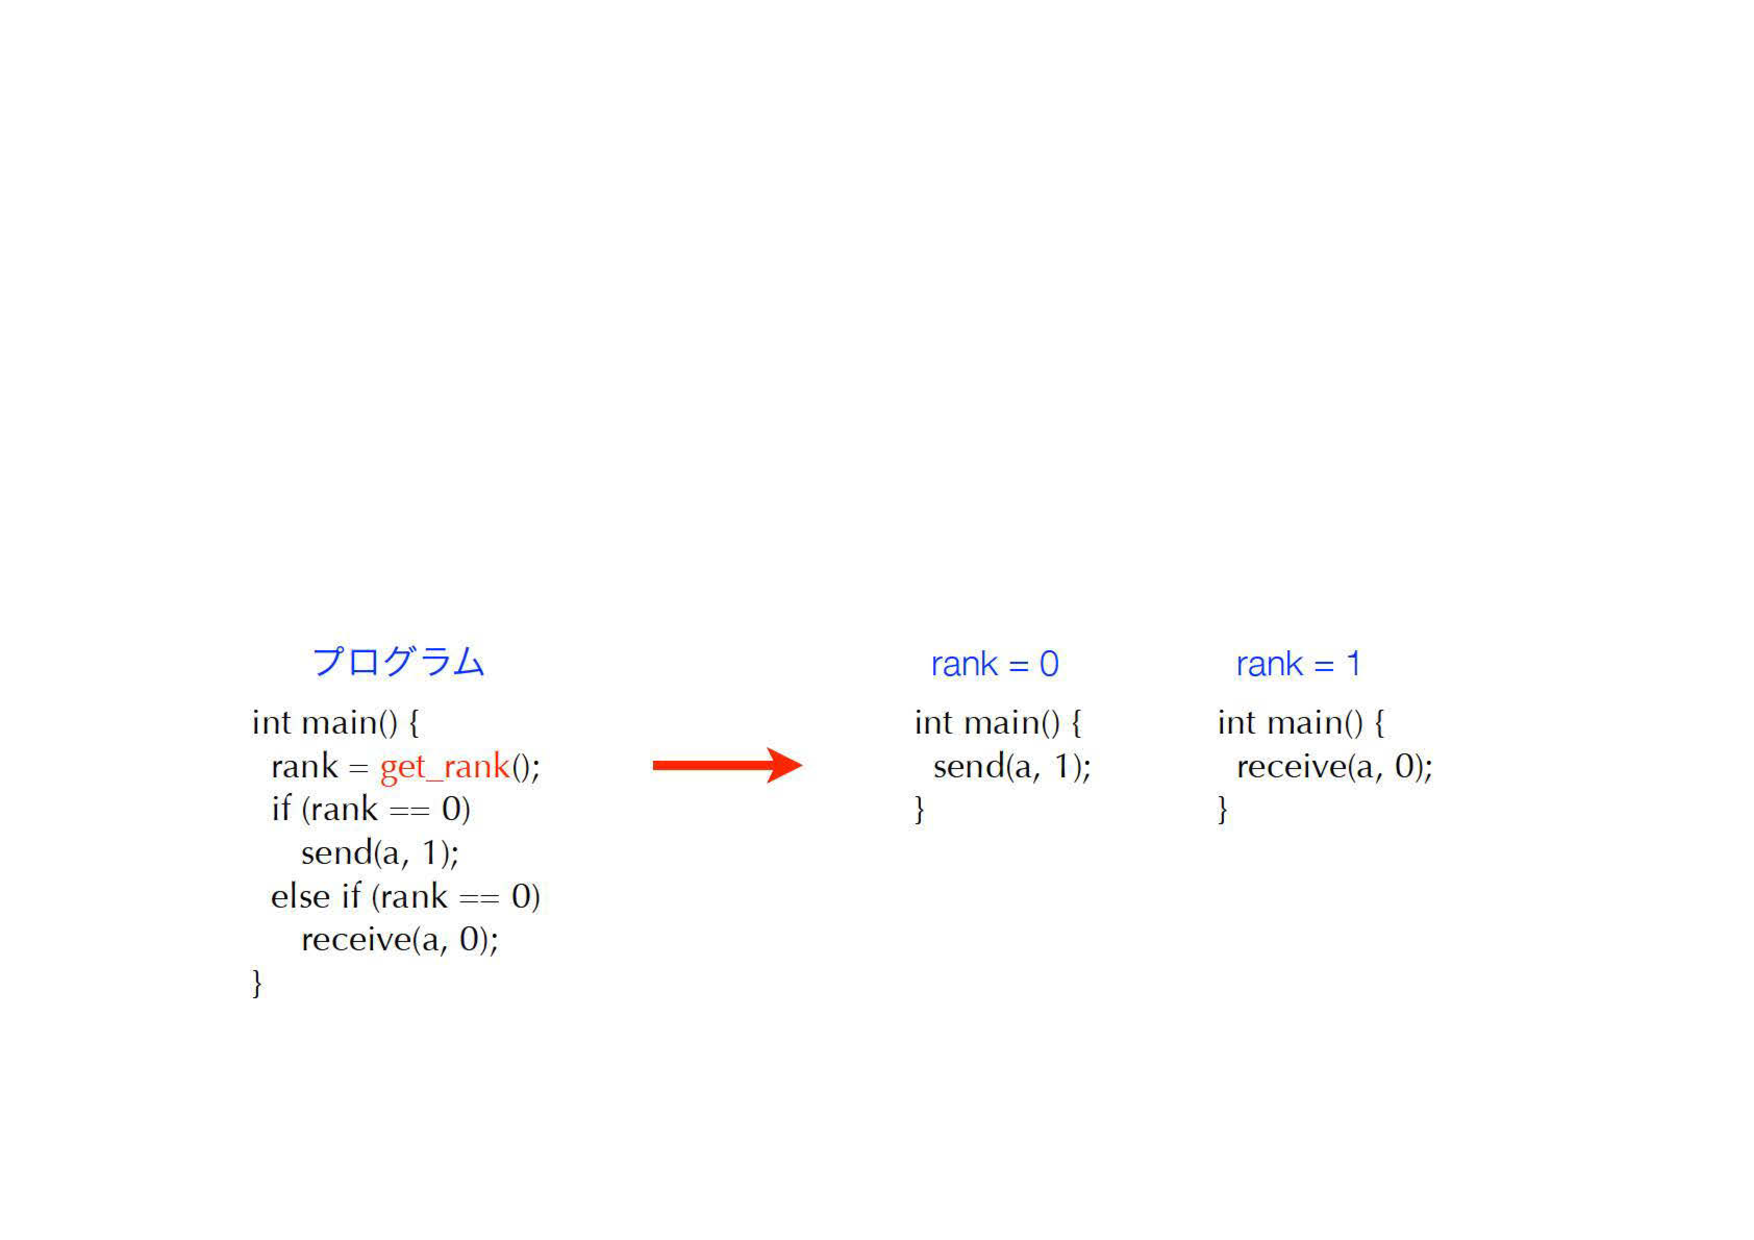
\includegraphics{image/spmd.pdf}}
  \end{itemize}
\end{frame}

\begin{frame}[t,fragile]{アムダール(Amdahl)の法則}
  \begin{itemize}
    \setlength{\itemsep}{1em}
  \item 並列化による全体の性能向上率
    \[
    P = \frac{1}{X+(1-X)/n}
    \]
    $X$: 並列化されていない部分の実行時間の割合, $n$: ノード数
  \item $X$を限りなく零にしないと高並列ではすぐに性能が頭打ちに
  \end{itemize}
  \vspace*{-0em}\hspace*{1em}\resizebox{0.5\textwidth}{!}{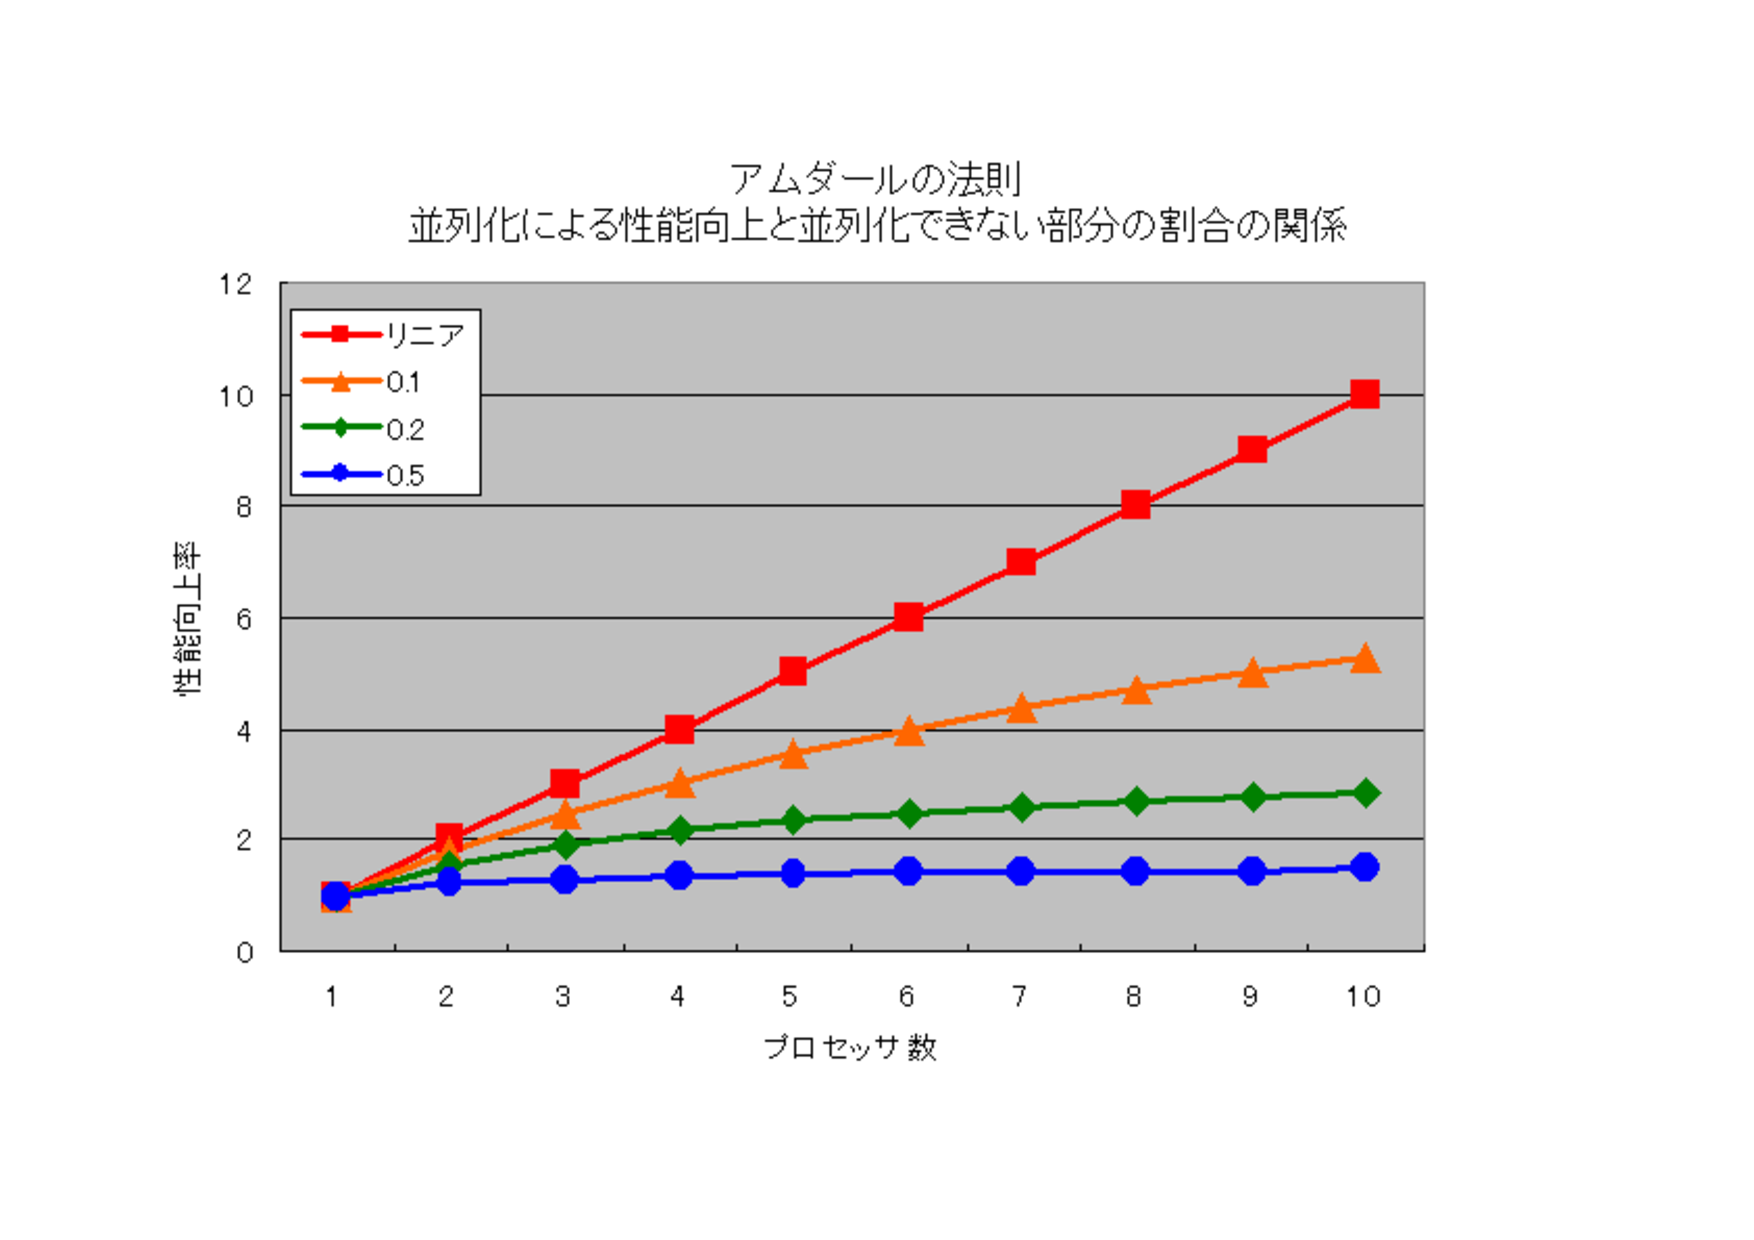
\includegraphics{image/Amdahl_law2.pdf}}
\end{frame}
